\documentclass[letterpaper, 11pt]{article}
\usepackage{comment} % enables the use of multi-line comments (\ifx \fi) 
\usepackage{fullpage} % changes the margin
\usepackage{fancyhdr} % for footer
\usepackage[UKenglish]{isodate}% http://ctan.org/pkg/isodate for date format
\usepackage{wrapfig}
\usepackage[font={small,sf}]{caption}
\usepackage{float}%force tables/figs into certain placement
\usepackage{graphicx}%for figures
\usepackage[leftcaption]{sidecap}%for figure captions
\usepackage{subcaption}%for figures
\usepackage{hyperref}%for hyperlinks
\usepackage[font=small,labelfont=bf]{caption}%for captions
\usepackage{natbib}	%for bibliography
\usepackage{placeins}%prevent images from floating into inappropriate sections
\usepackage{tabulary}%for table at the end, to get soft wrapping
%\usepackage[capbesideposition=inside,facing=yes,capbesidesep=quad]{floatrow}
\usepackage[]{textcomp}%for degree symbol
\usepackage{titlesec}%to change appendix headers
\usepackage[titletoc,toc,title]{appendix}%to change appendix headers

\usepackage{epigrafica}%changes default font to epigrafica
\usepackage[LGR,OT1]{fontenc}

\def\labelitemi{--}

\pagestyle{fancy}
\renewcommand{\headrulewidth}{0pt}

\lhead{}
\chead{}
\rhead{}
\lfoot{Frost Entomological Museum}
\cfoot{}
\rfoot{\thepage}
\renewcommand{\footrulewidth}{0.4pt}
\title{\textbf{DRAFT} Collection Management Policy}
\author{Frost Entomological Museum Curator \& Interest Group}

\begin{document}
\cleanlookdateon %removed ordinal date
\maketitle
\thispagestyle{fancy}

\section*{Preamble}
This Collection Management Policy (CMP) document outlines the mission, responsibilities, and collections policies of the Frost Entomological Museum at Penn State. Definitions of important terms are provided in Appendix \ref{app:definitions}. Collections management procedures---that is, the fine scale details regarding collection activities, including step-by-step protocols, vendor list, \textit{etc}.---are described separately as a collection of Frost Museum Standard Operating Procedures (Frost SOPs).\\

\begin{figure}[ht!]
    \centering
    \begin{subfigure}[ht!]{0.43\textwidth}
        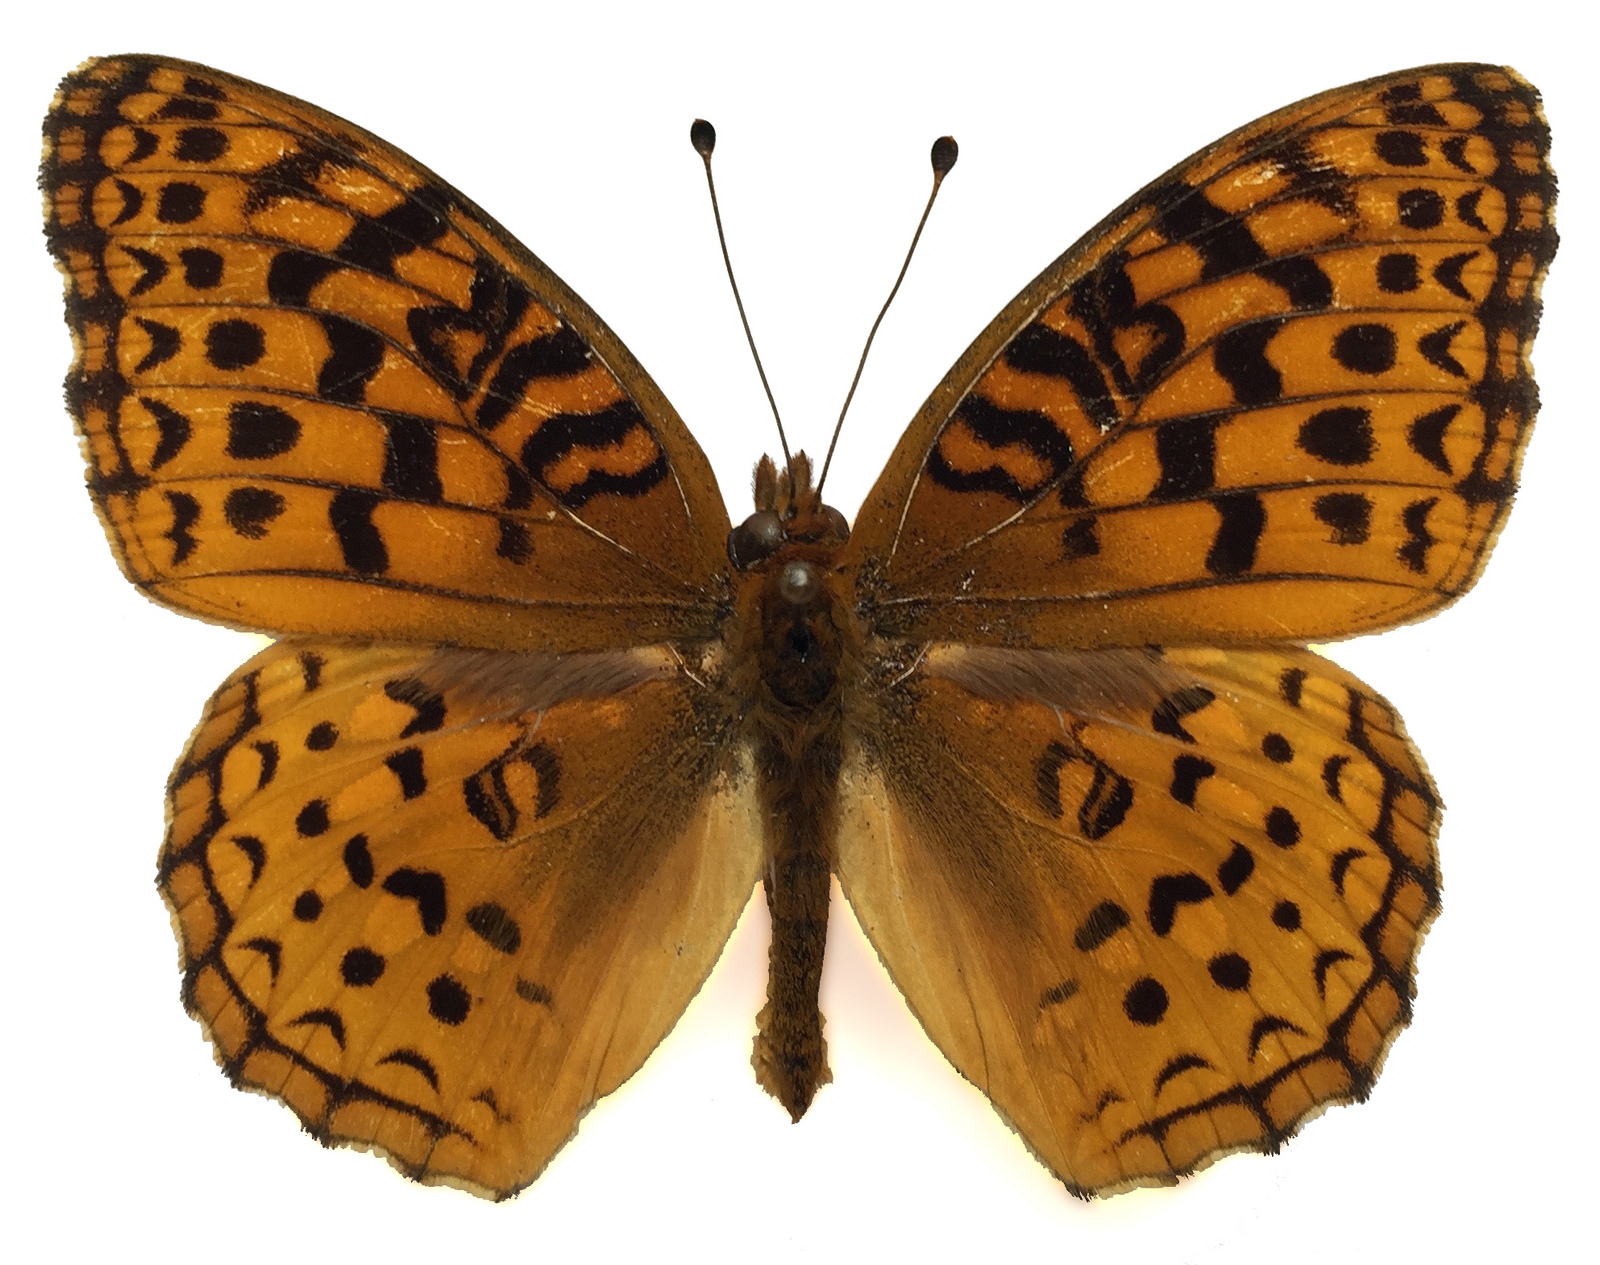
\includegraphics[width=\textwidth]{butterfly}
    \end{subfigure}
    \qquad
    \begin{subfigure}[ht!]{0.45\textwidth}
        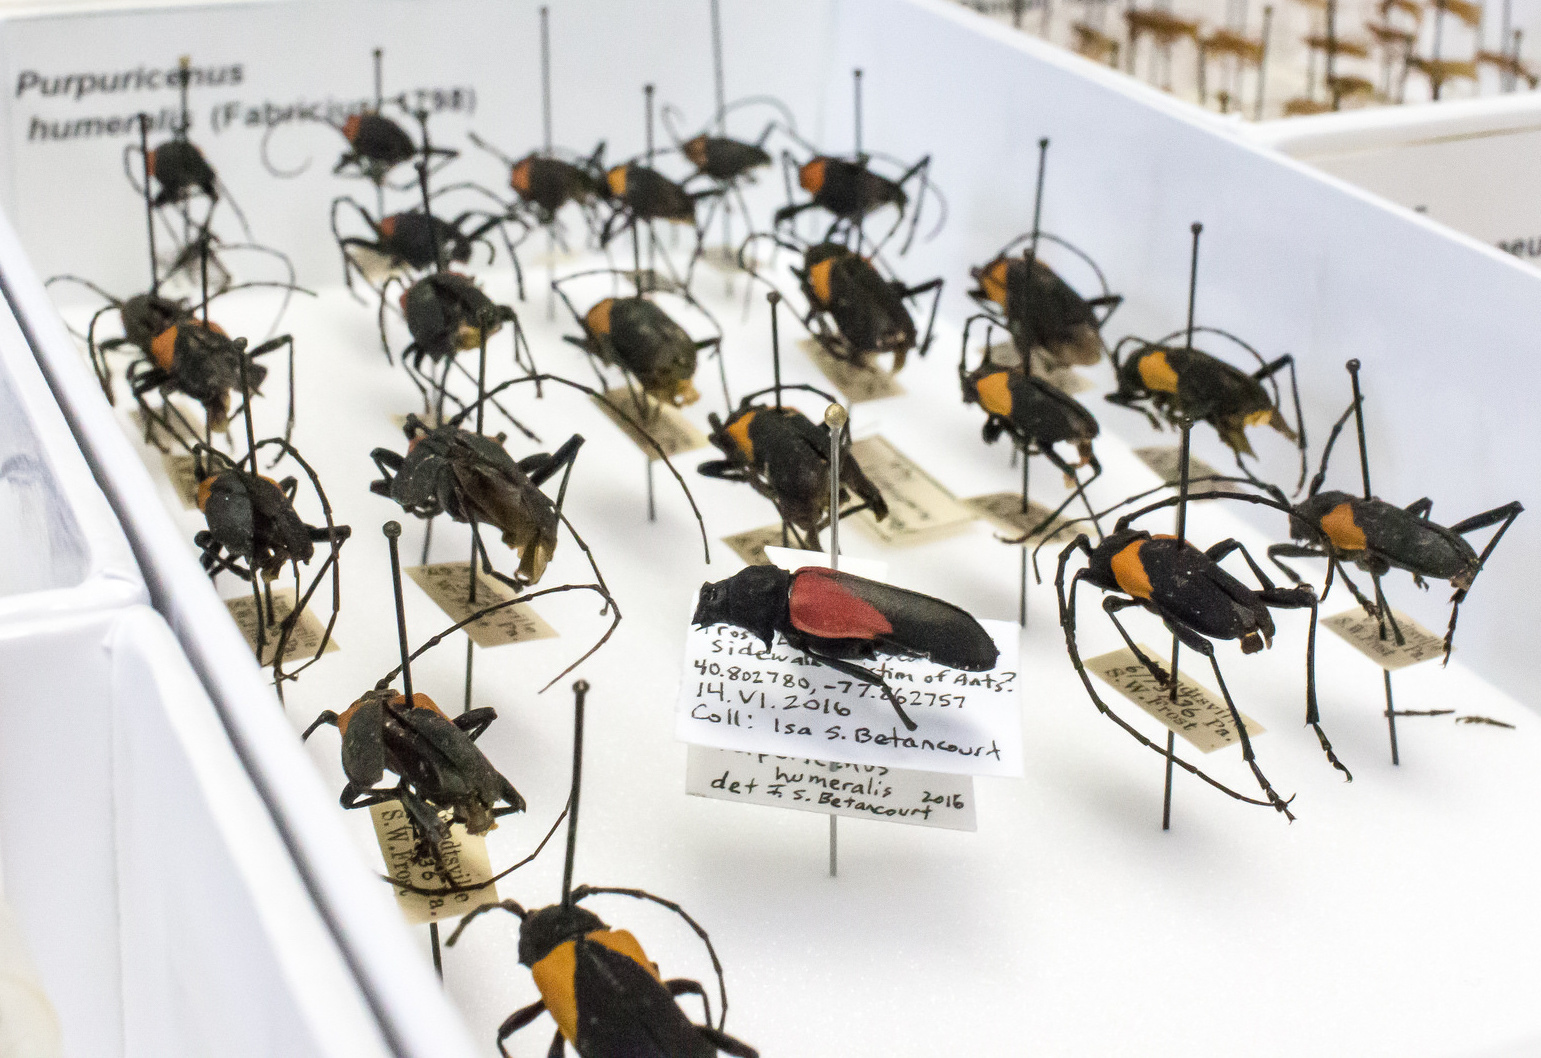
\includegraphics[width=\textwidth]{pinned}
    \end{subfigure}
    \caption{Frost Entomological Museum specimens. Photos CC BY 2.0 by Andy Deans (L) and Isa Betancourt (R)}
\end{figure}

\section{Mission Statement}

The mission of the Frost Entomological Museum is to preserve in perpetuity the collections of the Department of Entomology at Penn State and its partners, to facilitate research on arthropods and on collections practices, to disseminate research results broadly, to serve as a resource for science education and training, to foster a sense of curiosity about the natural world, and to instill responsibility in all people to make our world a better place.

\clearpage
\section{Statement of Authority}
The Frost Entomological Museum is housed within the Department of Entomology, College of Agricultural Sciences, at the Pennsylvania State University (University Park campus). A \textbf{Museum Committee}, known historically as the Frost Museum Curator \& Interest Group, is appointed annually by the Department and always includes (minimally) the Director, the Collection Manager, at least one student, and two other members. The Museum Committee has the authority and responsibility to make decisions regarding the acquisition, accession, accessibility, deaccession, and disposal of objects in the collection. The Museum Committee also makes decisions regarding changes in collection policies and procedures. Decisions made by the Museum Committee are determined by a majority vote. The University, College, and Department respect the professional expertise and views of the Museum staff in fulfilling the Museum's mission.%\footnote{See Appendix \ref{app:definitions} for descriptions of committee and personnel titles, as well as definitions for important terms}
\\

\noindent{}The \textbf{Director}, known historically as ``Curator'', is responsible, in part, for:
\begin{enumerate}
\item Providing leadership on Museum policy, program direction and planning, and securing budget support to carry out the collections management requirements established in this document
\item Providing leadership in developing and implementing a long-term collections plan that provides a framework for making collection development, acquisition, management, and disposals decisions
\item Assuring compliance with institutional, state, national, and international laws, as well as natural history collections best practices
\item Establishing metrics for monitoring and reporting progress towards implementation of collections management standards
\item Making sure that all Museum employees and affiliates are trained in current procedures, safety protocols, and relevant museum best practices
\end{enumerate}

\noindent{}The \textbf{Collection Manager}, known historically as ``Assistant Curator'', is responsible, in part, for:
\begin{enumerate}
\item Providing feedback on Museum policy, program direction and planning, and budget requirements for carrying out the collections management activities established in this document
\item Providing feedback on developing and implementing a long-term collections plan
\item Assuring compliance with institutional, state, national, and international laws, as well as natural history collections best practices
\item Providing feedback on metrics for monitoring and reporting progress towards implementation of collections management standards
\item Facilitating the training of Museum employees and affiliates in current procedures, safety protocols, and relevant museum best practices
\item Refining and implementing the Frost Entomological Museum Collections Management Procedures (``Frost SOPs'')
\end{enumerate}

\clearpage
\section{Scope of the collections}
\subsection{Kinds of objects}
The collections housed at the Frost Entomological Museum primarily include:
\begin{itemize}
\item Specimens, especially insects (Hexapoda) and other terrestrial arthropods (mainly Myriapoda and Arachnida), including their traces (exuviae, for example), plant parts that instantiate insect damage or modification (galls and leaf mines, for example), and insect nests
\item Paper-based resources that relate to entomological collections, including books, maps, printed photographs, field notes, lab notes, and correspondence
\end{itemize}

\subsection{Kinds of collections}
Specimens housed at the Frost Entomological Museum are partitioned across three primary collections:
\begin{enumerate}
\item Research - This collection includes all types, vouchers, and specimens highly valued for their real and potential contributions as data and metadata for research
\item Teaching - This collection includes specimens with limited research potential but high value as instances of certain taxa, phenotypes, and other biological phenomena. This collection primarily serves the Insect Biodiversity and Evolution (ENT 432) course
\item Outreach - This collection includes specimens with limited research potential, in most cases, but high value as objects that inspire and educate people about entomology and insects
\end{enumerate}

\subsection{Specimen preservation types and limitations}
The Frost Entomological Museum primarily cares for specimens preserved in alcohol or other liquid preservative, specimens preserved as slide mounts (Canada balsam or other archival medium), and dried specimens on pins or in envelopes (Odonata). There is limited cold storage (-80\textdegree{}C). The Museum does not maintain cultures of live organisms.

\subsection{Geographical limits}
The geographic scope of the collection is global.

\subsection{Chronological limits}
There are no chronological limits to the collection, although the vast majority of specimens are from the Anthropocene.

\clearpage
\section{Collections management activities}
\subsection{Acquisitions}
Specimens and associated objects are added to the collections in a variety of ways, including transferral by government agency, purchase (very rare), collection by researchers and students, or receipt as exchanges, gifts, or bequests.

\subsubsection{General criteria for acquisition}
Only specimens, collections, and associated objects that meet the following criteria are eligible for acquisition: 
\begin{enumerate}
\item Specimens are consistent with the collection goals and scope of the Museum as stipulated in this Collections Management Policy document
\item The provenance of the specimens is adequately documented (see \ref{sec:provenance}), and the donor/conveyor can demonstrate that the specimens were collected legally
\item The donor/conveyor declares full and clear legal title or the right to transfer full and clear legal title of the collections and all associated materials offered
\item Adequate scientific documentation accompanies the specimen(s) and/or the specimens offer extraordinary value for the Teaching and Outreach collections
\item Sufficient physical, personnel, and monetary resources are available to care for the specimens once they are accepted. Because of its fiduciary responsibility to maintain and preserve objects in perpetuity for the common good, the Museum will not acquire objects for which it is unable to provide adequate space, financial resources for care and conservation, and appropriate staff (curatorial, collection management, conservation, preservation and registration).
\item The specimens are not encumbered with unusual conditions set by the donor/conveyor
\end{enumerate}

\noindent{}The Museum Committee is required to consider and approve or decline all significant donations, here defined as collections with \textgreater100 specimens or which require more than one drawer or one slide tray or jar to house. As a general rule, no specimen or associated object shall be acquired unless there is a good faith intention to retain it for the collections for the foreseeable future. Exceptions---for example if the collection is of mixed quality---will be communicated in writing to the donor prior to acquisition of the collection.

\subsubsection{Acceptable provenance}\label{sec:provenance}
Before approving the acquisition of a specimen or a collection of specimens and associated objects, the Museum has the responsibility, in good faith, to ascertain from the circumstances surrounding the transaction, or knowledge of the specimen's or collection's provenance, that it was not stolen or wrongfully converted, and that it is not illegally present in the United States. The Museum also has the responsibility to ascertain that any proposed new acquisition was not unethically acquired from its source, unscientifically documented, or illegally removed from its country of origin. A signed Deed of Gift form (see \ref{sec:deedsofgift}) or letter with similar information is required for all gifts that originate from outside the Department.\\

\noindent{}Museum will not accept abandoned objects, except under extreme circumstances and with the written approval of the Museum Committee. As clear title cannot be ascertained, it is unwise to accept any abandoned object. Property brought to the Museum and abandoned will not be accepted.

\subsubsection{Deeds of gift}\label{sec:deedsofgift}
The Museum will obtain a signed Deed of Gift (and/or other relevant legal documents) from a donor whenever any specimens, related objects, or equipment are received for accessioning from outside the Department of Entomology. This ensures that the donor is giving the objects to the Museum irrevocably and unconditionally and that the donor owns and has acquired the objects legally. When the donor-signed Deed of Gift form is returned, the official accession forms and an acknowledgment from the Director will be generated and copies sent to the donor. The Museum accepts only unrestricted donations, unless the Museum Committee allows an exception for an extraordinary collection, under extraordinary circumstances.

\subsubsection{Appraisals}
Appraisals required for tax deduction purposes are the responsibility of the donor. Museum and affiliated staff may not provide appraisals.

\subsubsection{Permits and restrictions}
The collection, importation, exportation, and interstate shipment of many kinds of specimens (including entomological) may be regulated by state, Federal, and foreign statutes. The Federal laws involved include, but are not limited to, the Lacey Act, the Endangered Species Act of 1973, as amended, the Convention on International Trade in Endangered Species of Wild Flora and Fauna, and the Antiquities Act.\\

\noindent{}The Director and Collection Manager are responsible for assuring compliance with these laws and regulations and for informing Museum staff about these issues. Specimens collected under permits with restrictions---for example, if primary types must be deposited in the country of origin---must be labeled accordingly. 

\subsection{Deaccession/disposal}
As defined in this document, deaccessioning is the formal process used to permanently remove an accessioned specimen from the collections. Disposal here refers to the removal of a specimen that was never formally accessioned into the research collection.

\subsubsection{General criteria for deaccession/disposal}
Specimens may be deaccessioned by mutual agreement between the Director and Collection Manager if they are not encumbered with restrictions and meet at least one of the following criteria:
\begin{itemize}
\item They are no longer germane or useful to the purposes and activities of the Museum
\item They are cannot be preserved properly
\item They have deteriorated beyond usefulness
\item They lack sufficient documentation to make it scientifically useful or the existing documentation requires substantial staff time and resources to reconcile (for example, vials are labeled only with codes, and the collecting event data are in a spreadsheet)
\item They are redundant
\item They can be put to better use in another educational/research organization
\item They occupy space and use valuable resources that could better be used to improve or strengthen another area of the collections in order to further the Museum's mission and goals
\item They must be repatriated it to their country of origin
\item The number under consideration is fewer than 100
\end{itemize}

\noindent{}Assemblages of more than 100 specimens that fit a common theme---for example, from same project, collecting event, or of the same taxon---and which are being considered for deaccessioning or disposal require approval from the Museum Committee.\\

\noindent{}Specimens deemed inappropriate for the collection may be disposed of in a variety of ways, including transfer to another collection and/or donation to another research or educational enterprise. Primary type specimens (holotypes, lectotypes, neotypes, and syntypes) cannot be exchanged, but may be repatriated if collected contrary to the laws of its country of origin and if recommended by the Museum Committee. The sale or exchange of specimens with non-researchers and non-cultural/non-scholarly entities is highly discouraged.\\

\noindent{}Specimens that are to be deaccessioned should be imaged (if time and resources permit), and all catalog numbers (identifiers) recorded in the database as ``deaccessioned'', with the new repository recorded.

\subsection{Inventory}
The Director and Collection Manager will maintain an approximate inventory of all collections (until such time that they are completely digitized/cataloged) and a detailed inventory of significant equipment---microscopes, cameras, collecting gear, for example---not already accounted for by the Office of Physical Plant (OPP).

\subsection{Access}
The Museum strives to provide full, open and equal access to collections, including associated data, and yet balance restraints imposed by security considerations, specimen and object fragility, and staff limitations, including research in progress by Museum staff and affiliates. Members of the public are allowed supervised access to conduct specific research or to participate in prearranged educational tours. Access to the collections will be denied to individuals who have little or no documented previous experience with entomological research collections or who have failed to handle specimens in accordance with departmental procedures and standard professional practices, as verified by the appropriate contact person, the Collections Manager, or Director.

\subsection{Loans}
The Museum lends specimens to researchers and educational organizations for scientific study, identification, and exhibition. The Museum, through its researchers, students, and staff, borrows specimens for scientific study, identification, and, on occasion, in contemplation of an exchange. When researchers, staff, associates, and other long-term visitors leave the department (retirement, resignation, or new position, for example) they must follow the Exit Protocols and Exit Clearance Procedures (See SOP \#???).%create this!

\subsubsection{Outgoing Loans}
The Director or Collection Manager may initiate an outgoing loan in response to a loan request or at his/her own discretion---for example, for identifications of research collection specimens by specialists. Loans of substantial quantities of specimens, or substantial value, or specimens that may need special care or handling, or those involving special conditions are subject to Museum Committee recommendation of approval. Loans are not issued to students; instead, these loans are assigned to the student's major professor at an institution and only if the latter can vouch for the professionalism of the student in writing. Specimens from the Research collection are generally not loaned for exhibition.\\

\noindent{}Prior to shipment or transfer, a condition report is made by the Collection Manager. This report includes a list of the specimen identifiers and the condition of the specimens; the report shall be maintained in the collection database. Outgoing loans shall be for a specific period of time, typically a year, subject to renewal if desired. The Collection Manager or Director may extend the loan at his/her discretion. Loans are not shipped between late November and the end of December.\\

\noindent{}Publications derived from examination or other use of Museum specimens must acknowledge the Frost Entomological Museum.

\subsubsection{Incoming Loans}
Packages containing specimens on loan to Museum researchers or specimens to be returned to the Museum's collections must be freeze-treated upon arrival. The loan initiator (if incoming loan) or Collection Manager (if package is loan being returned) must then document the state of the specimens and process appropriate paperwork (with copies loaded into the Museum database). Each specimen that is on loan from another institution must be labeled with the loaning institution's coden and the loan number. Loans must be returned prior to the expiration of the loan, unless an extension is secured from the loaning institution. The Frost Entomological Museum requests that loan returns, especially those with type specimens, not be shipped late November and late December. Matters of provenance shall be considered by Museum researchers before a loan is requested.

\subsubsection{Packing and Shipping}
The Collection Manager is responsible for packing outgoing shipments or inspecting the packing by other Museum employees. Packing and shipping best practices will be used to ensure the safety and security of specimens.

\subsubsection{Policy on retention of duplicate specimens}
To promote wide dissemination of biodiversity knowledge and data that is ultimately derived from voucher specimens, the Frost Entomological Museum is willing to donate specimens to other museums and specialists collaborating with the Museum in the development of its collections. For specimens already determined to species, specimens may be exchanged. Exchanges must be beneficial to both institutions. Specimens representing unique data points will not be exchanged. \\

\noindent{}For undetermined material, duplicates (usually from series with the exact same data) may be retained in recognition of services performed. In determining the appropriate number of duplicates to be retained, consideration will be given to the level of identification provided, the level of preparation performed, and the source of the request for services. The following provides guidelines, and exceptions may be made with the recommendation of the Museum Committee. 
\begin{enumerate}
\item When specimens are prepared and identified with reasonable certainty to species, a proportion of duplicate specimens---with written permission from the Director and/or Collection Manager---will be eligible for retention by the preparer.
\begin{itemize}
\item If the material was prepared (pinned, spread, slide-mounted, \textit{etc}.) from a bulk sample by the borrower, then up to 50\% of the series may be retained
\item If the material was prepared prior to loaning and the request for identification was made by the Director or Collection Manager, then up to 33\% of the series may be retained
\item If the material was already prepared and the loan was made at the request of the retainer, then up to 25\% of the series may be retained.
\end{itemize}
\item When the portion of specimens to be retained is fractional, the number may be rounded up (for example, 25\% of 2 is half a specimen, so 1 specimen may be retained).
\item The retainer will prepare a list of taxon determinations, specimen label data, sex determinations, and identifiers for the specimens to be retained. This information is then returned to the Museum, along with the other identified specimens. Upon receipt of these specimens the Museum will register the desired specimens as a gift to the retainer.
\item When the specimens are part of a type series (actual or to be designated), the number of specimens to be retained will be negotiated on a case-by-case basis, independent of the above rules.
\end{enumerate}

\subsection{Care and control of collections}
The Director is ultimately responsible for insuring the safety and well-being of the collections. These objectives, however, require the conscientious assistance of all Museum employees and visitors. Staff members, associates, students, visitors, and resident affiliate staff are expected to be aware of their general duty to preserve, protect, and control collections and related objects at all times.\\

\noindent{}The Director and Collection Manager shall periodically evaluate---with appropriate Penn State support---offices, security, fire, safety, and hazard controls within the Museum. Special attention shall be given to these matters during periods of renovation or construction, and it is the responsibility of the Director and Collection Manager to coordinate with the Department and Office of Physical Plant (OPP) in a clear and timely manner.\\

\noindent{}The Museum uses its Collections Standards documentation (SOP \#???) %refer to profiling scheme!
as part of its collections management procedures. These criteria set forth standards for meeting management and conservation needs of departmental collections and related objects. Every effort shall be made to reorganize and/or obtain additional storage space that is adequate, secure, and of such quality as to meet specimen preservation and retrieval needs as the collections grow. The Museum uses USNM standards for dry storage.\\

\noindent{}The Director and Collection Manager are responsible for knowing the current location of family-level and type collections entrusted to their care. Any movement of such a unit from its assigned location shall be made only after mutual agreement between the Director and Collections Manager. Specimens are arranged alphabetically by family, genus, and species within each order.

\subsubsection{Destructive sampling}
Routine requests to destructively sample specimens, including genitalia dissections and DNA extraction, must be approved by the Director or Collection Manager. Large scale or otherwise unusual requests will be referred to the Museum Committee. Approval of requests depends on the following criteria:
\begin{itemize}
\item Scientific value the project
\item Feasibility of the project
\item Qualifications of the investigator(s)
\item Evidence of sufficient lab facilities and resources
\item Appropriateness of requested specimens for the study
\item Amount of sampling or tissue needed
\item Reasons why samples could not be obtained from the field or other institutions
\item Appropriate laws and conditions described by collecting permit(s)
\end{itemize}
\noindent{}If the borrower is granted permission to sample destructively s/he agrees to the following conditions:
\begin{itemize}
\item No part or by-product, including extracted DNA, may be loaned or given to another researcher or institution without written permission from the Director
\item No commercial use of the sample will be made without prior approval, including licenses or patents based on samples or byproducts, or any information derived from them
\item Publications that result from tissues and other parts obtained from Museum specimens must specifically acknowledge the Museum and incorporate any other acknowledgments that might be required by the original collector (this may include acknowledging the grants that made the acquisition of the sample possible) or collecting permits
\item Sequences obtained from Museum specimens must be deposited in a public genetic database when the research has been submitted or accepted for publication, and the accession numbers must be sent to the Collection Manager
\item Dissected parts must be reassociated with the original specimen, for example in a genitalia vial with glycerol
\item Unused DNA or other extract must be returned to the Museum upon completion of the research, unless otherwise agreed upon in writing by the director
\end{itemize}

\subsubsection{Use of collections as a reference}
Objects may occasionally be brought to the Museum for identification. Museum staff reserve the right, however, to decline to interact with these objects and their owners. If an object is to be left at the Museum it must be recorded as an unsolicited loan to the Collections Manager (or Director if appropriate), and include the owner's name, address, and the reason for leaving the object. Failure to remove the object by the stated reclamation date may result in its disposal or treatment as abandonment (subject to accessioning into the collection). Identification or authentication services are generally not provided for any commercial purpose. Museum staff will not authenticate any objects for other persons or agencies under circumstances that could encourage or benefit illegal, unethical, or irresponsible traffic in such materials. 

\subsubsection{Special uses of collections}
\paragraph*{Promotions.} Objects in the collections may be used for promotion of the Museum, Department, College, or University only after written approval has been obtained from the Director.

\paragraph*{Exhibition.}
With the written approval of the Director and Museum Committee, certain collection objects may be available for exhibition within the Museum or in partnership with another institution. All of these objects must be formally accessioned (they bear unique identifiers and are in the Museum database) and clearly labeled as property of the Frost Entomological Museum. Appropriate environments and care must be applied in displaying these objects and all loan procedures must be followed for each object. Objects may be recalled at any time by the Director. 

\paragraph*{Inspiration.}
Use of specimens in the Outreach and Teaching collections as objects of inspiration, for example by students in art classes or by individual artists visiting the Museum, is encouraged. Visits should be coordinated with the Collection Manager or Director, and approval is subject to the availability of staff and other resources. Specimens in the Research collection are generally not available for non-research purposes.

\subsection{Risk Management and Security}
\subsubsection{Disaster preparedness}
The Director and Collection Manager are responsible for developing the Disaster Preparedness plan, which is approved by the Museum Committee.
\subsubsection{Building security}
Exterior doors are to be kept locked at all times, except for the front door during hours that the Museum is open. Staff and affiliates who require keys must pass an oral exam administered by either the Director or the Collection Manager; keys will not be awarded until the applicant can answer all questions correctly.

\clearpage
\section{Ethics and standards of conduct}
\subsection{Code of ethics}
The Frost Entomological Museum adheres to the code of ethics as adopted by the American Alliance of Museums\citep{AAMethics} and is bound by the Pennsylvania State University ethics statements and policies\citep{PSUethics}. The Museum also complies with all applicable local, state, and federal laws, international conventions, and legal standards governing trust responsibilities. 

\subsection{Personal Collections}
Staff must not personally compete with the Frost Entomological Museum for acquisitions in which the Museum has formally declared an interest. No staff members may use their museum affiliation to promote their personal collecting activities or those of an associate's. It is the responsibility of the Museum staff owning such collections to demonstrate to the satisfaction of their supervisors that they are not expanding, enhancing, or in any way competing with any function of the Museum to further such activities.\\

\noindent{}Although many specimens are held in an unaccessioned state pending completion of studies or preparation, it is understood that any such specimens obtained through gift, exchange, or individuals conducting field collecting while in the employ of the Museum or Department is presumed to be the property of the Department, or of the affiliate organizations, and shall be treated accordingly.

\noindent{}Objects belonging to staff members may be loaned to the Museum for exhibition or research if the item(s) would significantly enhance the educational value of the larger exhibition or research question. There cannot, however, be a conflict of interest, or even a perceived conflict of interest, wherein the staff member may personally benefit from such a loan. Prior to the use of objects belonging to staff or private individuals, there must be approval from the Museum Committee.

\subsection{Intellectual property rights}
The Frost Entomological Museum adheres to Penn State's Position on Intellectual Property\citep{PSUintellectual}, including Policies IP01 and IP06:
\begin{itemize}
\item \url{https://guru.psu.edu/policies/ip01.html}
\item \url{http://guru.psu.edu/policies/IP06.html}
\end{itemize}

\clearpage
\section{Revising, licensing, and availing this document}
This Collections Management Policy document should be reviewed by the Museum Committee every five years to assure compliance with the latest Penn State policies and collections best practices and policies.\\

\noindent{}The most recent approved version of this document will be published on the Museum website and availed under a (CC0 1.0) license. Readers can copy, modify, distribute and perform the work, even for commercial purposes, all without asking permission.

\clearpage
\section*{Acknowledgments}
The development of this collections management policy (CMP) document relied heavily on established policies (and wording) developed for other institutions, especially the National Museum of Natural History (Smithsonian)\citep{NMNHpolicy}, including its Department of Entomology CMP\citep{NMNHEntpolicy}, the Natural History Museum in London\citep{NHMpolicy}, Museum of Comparative Zoology (Harvard)\citep{MCZpolicy}, the Utah Museum of Natural History CMP \citep{UtahCMP}, KU's Mammalogy Division destructive sampling policy\citep{KUmammals}, Penn State's EMS Museum and Art Gallery\citep{PSUEMS}. We thank Julianne Snider, Dana Carlisle Kletchka, Dave Furth, and Floyd Shockley for providing vital information.


\clearpage
\titleformat{\section}{\normalfont\Large\bfseries}{\appendixname~\thesection.}{1em}{}


\begin{appendices}
\section{Definitions}\label{app:definitions}
\begin{description}
  \item[Accession] is the formal process by which a specimen receives a unique identifier and is entered into the database.
  \item[Coden] is a unique string of three or four letters that refers to a collection. The Frost Museum's coden, as assigned in \cite{coden}, is PSUC.
  \item[Collections management] is the deliberate development, maintenance, preservation, documentation, use and disposition of collections. Collections include objects, natural specimens, representational samples, artifacts, information about and derived from such holdings, and other items that are acquired, preserved and maintained for pubic exhibition, education, and study.
  \item[Collections Management Policy] is a document that provides guidelines so that decisions concerning collections are prudent, responsible, informed, and in accordance with NMNH’s mission and the Institution’s policies and mission. A policy ensures collections are responsibly developed, maintained, exhibited, used, loaned, and preserved. The policy is separate and distinct from the procedures and mechanisms used to implement policy.
  \item[Collections Management Procedures] document directly implements the collections management policy (CMP) and guides staff members day-to-day as they administer collections. This document is also referred to as the ``Frost Standard Operating Procedures'', or ``Frost SOPs''.
  \item[Deaccession] is the formal process by which an accessioned specimen is marked in the Museum database as no longer being part of the Museum. The specimen's disposition is also recorded, and the specimen is physically removed from the collection.
  \item[Museum Committee,] also known as the Frost Museum Curator \& Interest Group, is appointed annually by the Department and always includes (minimally) the Director, the Collection Manager, at least one student, and two other members. The Committee is charged with making decisions regarding the safety, growth, scope, and direction of the Museum.
  \item[Types,] or type specimens, or type series refers to those specimens with special taxonomic relevance according to the International Code Zoological Nomenclature. Specimens designated as holo-, lecto-, or neotypes are especially important to the collection and are stored separately from other specimens.
  \item[Unique identifiers,] often referred to as ``catalog numbers'', are strings of numbers prefaced with PSUC\_FEM (for example, PSUC\_FEM 28711). Each string is unique within the collections of the Museum and provides a way to reference a single object.
\end{description}
\end{appendices}


\clearpage
% adding bibliography here
\bibliographystyle{unsrt}
\bibliography{bib}

\end{document}

\begin{figure}[ht!]
	\centering
  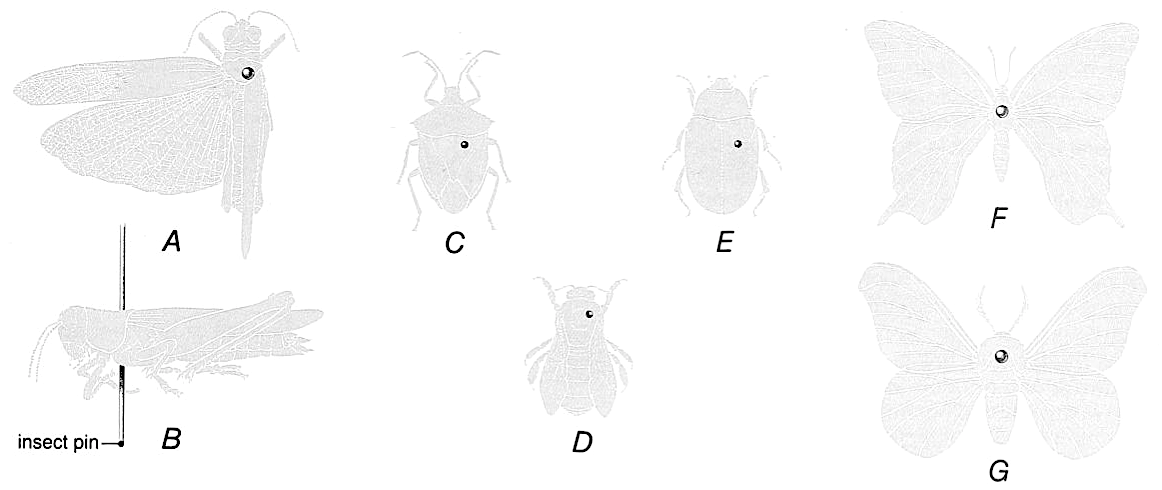
\includegraphics[width=0.75\textwidth]{PinsThorax}
  \caption{Ideal pin placement on different kinds of insects \citep[modified from][Fig. 17]{USDAmanual1986}}
  \label{pinthorax}
\end{figure}

\begin{figure}[ht!]
    \centering
    \begin{subfigure}[ht!]{0.43\textwidth}
        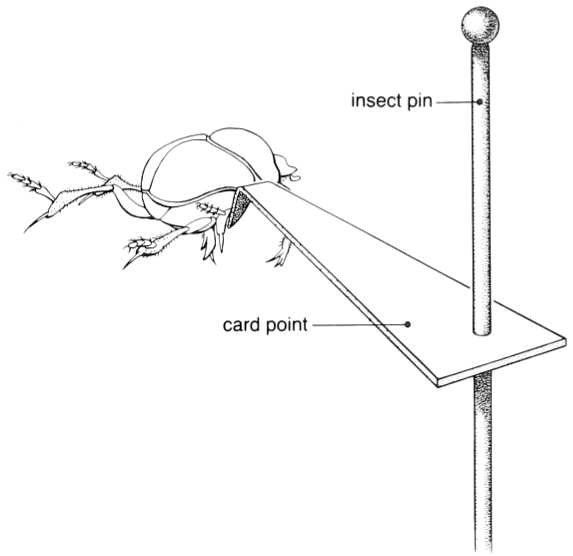
\includegraphics[width=\textwidth]{pointedBeetle}
        \caption{Coleopteran on point \citep[][Fig. 18C]{USDAmanual1986}}
        \label{fig:beetlepoint}
    \end{subfigure}
    \qquad
    \begin{subfigure}[ht!]{0.38\textwidth}
        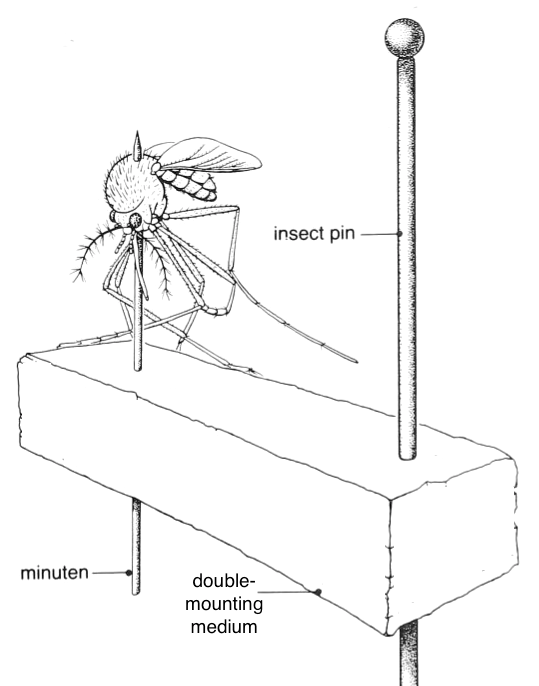
\includegraphics[width=\textwidth]{doublemount}
        \caption{Dipteran on point \citep[][Fig. 24]{USDAmanual1986}}
        \label{fig:flypoint}
    \end{subfigure}
    \caption{}
\end{figure}